\documentclass{beamer}
\usepackage[utf8]{inputenc}
\usepackage{graphicx, epsfig}
\usepackage{amsmath,mathrsfs,amsfonts,amssymb}
\usepackage{floatflt}
\usepackage{epic,ecltree}
\usepackage{mathtext}
\usepackage{fancybox}
\usepackage{fancyhdr}
\usepackage{multirow}
\usepackage{enumerate}
\usepackage{epstopdf}
\usepackage{multicol}
\usepackage{algorithm}
\usepackage[noend]{algorithmic}
\usepackage{tikz}
\usepackage{blindtext}
\usetheme{default}%{Singapore}%{Warsaw}%{Warsaw}%{Darmstadt}
\usecolortheme{default}

\setbeamerfont{title}{size=\Huge}
\setbeamertemplate{footline}[page number]{}

\setbeamertemplate{section in toc}[sections numbered]


\makeatletter
\newcommand\HUGE{\@setfontsize\Huge{35}{40}}
\makeatother    

\setbeamerfont{title}{size=\HUGE}
\beamertemplatenavigationsymbolsempty

% latin bold lower
\newcommand{\ba}{\mathbf{a}} 
\newcommand{\bc}{\mathbf{c}} 
\newcommand{\be}{\mathbf{e}} 
\newcommand{\bff}{\mathbf{f}} % \bf - for bold type
\newcommand{\bg}{\mathbf{g}} 
\newcommand{\bh}{\mathbf{h}} 
\newcommand{\bp}{\mathbf{p}} 
\newcommand{\bq}{\mathbf{q}} 
\newcommand{\bt}{\mathbf{t}} 
\newcommand{\bs}{\mathbf{s}} 
\newcommand{\bu}{\mathbf{u}} 
\newcommand{\bv}{\mathbf{v}} 
\newcommand{\bw}{\mathbf{w}} 
\newcommand{\bx}{\mathbf{x}} 
\newcommand{\by}{\mathbf{y}} 
\newcommand{\bz}{\mathbf{z}} 

% latin bold upper
\newcommand{\bA}{\mathbf{A}} 
\newcommand{\bB}{\mathbf{B}} 
\newcommand{\bC}{\mathbf{C}} 
\newcommand{\bG}{\mathbf{G}} 
\newcommand{\bI}{\mathbf{I}} 
\newcommand{\bJ}{\mathbf{J}} 
\newcommand{\bL}{\mathbf{L}} 
\newcommand{\bM}{\mathbf{M}} 
\newcommand{\bP}{\mathbf{P}}
\newcommand{\bQ}{\mathbf{Q}} 
\newcommand{\bR}{\mathbf{R}} 
\newcommand{\bT}{\mathbf{T}} 
\newcommand{\bU}{\mathbf{U}} 
\newcommand{\bV}{\mathbf{V}} 
\newcommand{\bW}{\mathbf{W}} 
\newcommand{\bX}{\mathbf{X}} 
\newcommand{\bY}{\mathbf{Y}} 
\newcommand{\bZ}{\mathbf{Z}} 

% latin cal upper
\newcommand{\cF}{\mathcal{F}} 
\newcommand{\cG}{\mathcal{G}} 
\newcommand{\cI}{\mathcal{I}} 
\newcommand{\cL}{\mathcal{L}} 
\newcommand{\cM}{\mathcal{M}} 
\newcommand{\cN}{\mathcal{N}} 
\newcommand{\cP}{\mathcal{P}} 
\newcommand{\cS}{\mathcal{S}} 
\newcommand{\cT}{\mathcal{T}} 
\newcommand{\cW}{\mathcal{W}} 
\newcommand{\cX}{\mathcal{X}} 
\newcommand{\cZ}{\mathcal{Z}} 

% latin bb upper
\newcommand{\bbE}{\mathbb{E}} 
\newcommand{\bbI}{\mathbb{I}} 
\newcommand{\bbP}{\mathbb{P}} 
\newcommand{\bbR}{\mathbb{R}} 

% greek bold lower
\newcommand{\bepsilon}{\boldsymbol{\epsilon}} 
\newcommand{\btheta}{\boldsymbol{\theta}} 
\newcommand{\blambda}{\boldsymbol{\lambda}} 
\newcommand{\bpi}{\boldsymbol{\pi}} 
\newcommand{\bmu}{\boldsymbol{\mu}} 
\newcommand{\bsigma}{\boldsymbol{\sigma}} 
\newcommand{\bphi}{\boldsymbol{\phi}} 

% greek bold upper
\newcommand{\bSigma}{\boldsymbol{\Sigma}} 

\DeclareMathOperator*{\argmin}{arg\,min}
\DeclareMathOperator*{\argmax}{arg\,max}

\newcommand{\createdgmtitle}[1]{\title[\hbox to 56mm{Deep Generative Models  \hfill\insertframenumber\,/\,\inserttotalframenumber}]
	{\vspace{1cm} \\ \textbf{Deep Generative Models} \\ {\Huge Lecture #1}}
	\author{Roman Isachenko}
		\institute{
\includegraphics[width=0.7cm]{../utils/aimasterslogo} \LARGE{AI Masters}}
	\date{2024, Summer}
}

\usepackage{tikz}
\usetikzlibrary{arrows,shapes,positioning,shadows,trees}

\newcommand\myfootnote[1]{%
  \tikz[remember picture,overlay]
  \draw (current page.south west) +(1in + \oddsidemargin,0.5em)
  node[anchor=south west,inner sep=0pt]{\parbox{\textwidth}{%
      \rlap{\rule{10em}{0.4pt}}\raggedright\scriptsize \textit{#1}}};}

\newcommand\myfootnotewithlink[2]{%
  \tikz[remember picture,overlay]
  \draw (current page.south west) +(1in + \oddsidemargin,0.5em)
  node[anchor=south west,inner sep=0pt]{\parbox{\textwidth}{%
      \rlap{\rule{10em}{0.4pt}}\raggedright\scriptsize\href{#1}{\textit{#2}}}};}
      
\AtBeginSection[]
      {
      	\begin{frame}{Outline}
      		\tableofcontents[currentsection]
      	\end{frame}
      }
      \AtBeginSubsection[]{
      	\begin{frame}{Outline}
      		\tableofcontents[currentsection,currentsubsection]
      	\end{frame}
}
\createdgmtitle{7}
\usepackage{tikz}

\usetikzlibrary{arrows,shapes,positioning,shadows,trees}
%--------------------------------------------------------------------------------
\begin{document}
%--------------------------------------------------------------------------------
\begin{frame}[noframenumbering,plain]
%\thispagestyle{empty}
\titlepage
\end{frame}
%=======
\begin{frame}{Recap of previous lecture}
	\begin{block}{Assumptions}
		\begin{itemize}
			\item Let $c \sim \text{Categorical}(\bpi)$, where 
			\vspace{-0.6cm}
			\[
			\bpi = (\pi_1, \dots, \pi_K), \quad \pi_k = P(c = k), \quad \sum_{k=1}^K \pi_k = 1.
			\]
			\vspace{-0.7cm}
			\item Let VAE model has discrete latent representation $c$ with prior $p(c) = \text{Uniform}\{1, \dots, K\}$.
		\end{itemize}
	\end{block}
	\begin{block}{ELBO}
		\vspace{-0.6cm}
		\[
			\mathcal{L} (\bphi, \btheta)  = \mathbb{E}_{q(c | \bx, \bphi)} \log p(\bx | c, \btheta) - {\color{olive} KL(q(c| \bx, \bphi) || p(c))} \rightarrow \max_{\bphi, \btheta}.
		\]
	\end{block}
	\vspace{-1.0cm}
	\[
		KL(q(c| \bx, \bphi) || p(c)) = - H(q(c | \bx, \bphi)) + \log K. 
	\]		
	\vspace{-0.5cm}
	\begin{block}{Vector quantization}
		Define the dictionary space $\{\be_k\}_{k=1}^K$, where $\be_k \in \bbR^C$, $K$ is the size of the dictionary.
		\vspace{-0.3cm}
		\[
		\bz_q = \bq (\bz) = \be_{k^*}, \quad \text{where } k^* = \argmin_k \| \bz - \be_k \|.
		\] 
		\vspace{-0.7cm}
	\end{block}
	\myfootnotewithlink{https://arxiv.org/abs/1711.00937}{Oord A., Vinyals O., Kavukcuoglu K. Neural Discrete Representation Learning, 2017} 
\end{frame}
%=======
\begin{frame}{Recap of previous lecture}
	\begin{figure}
		\centering
		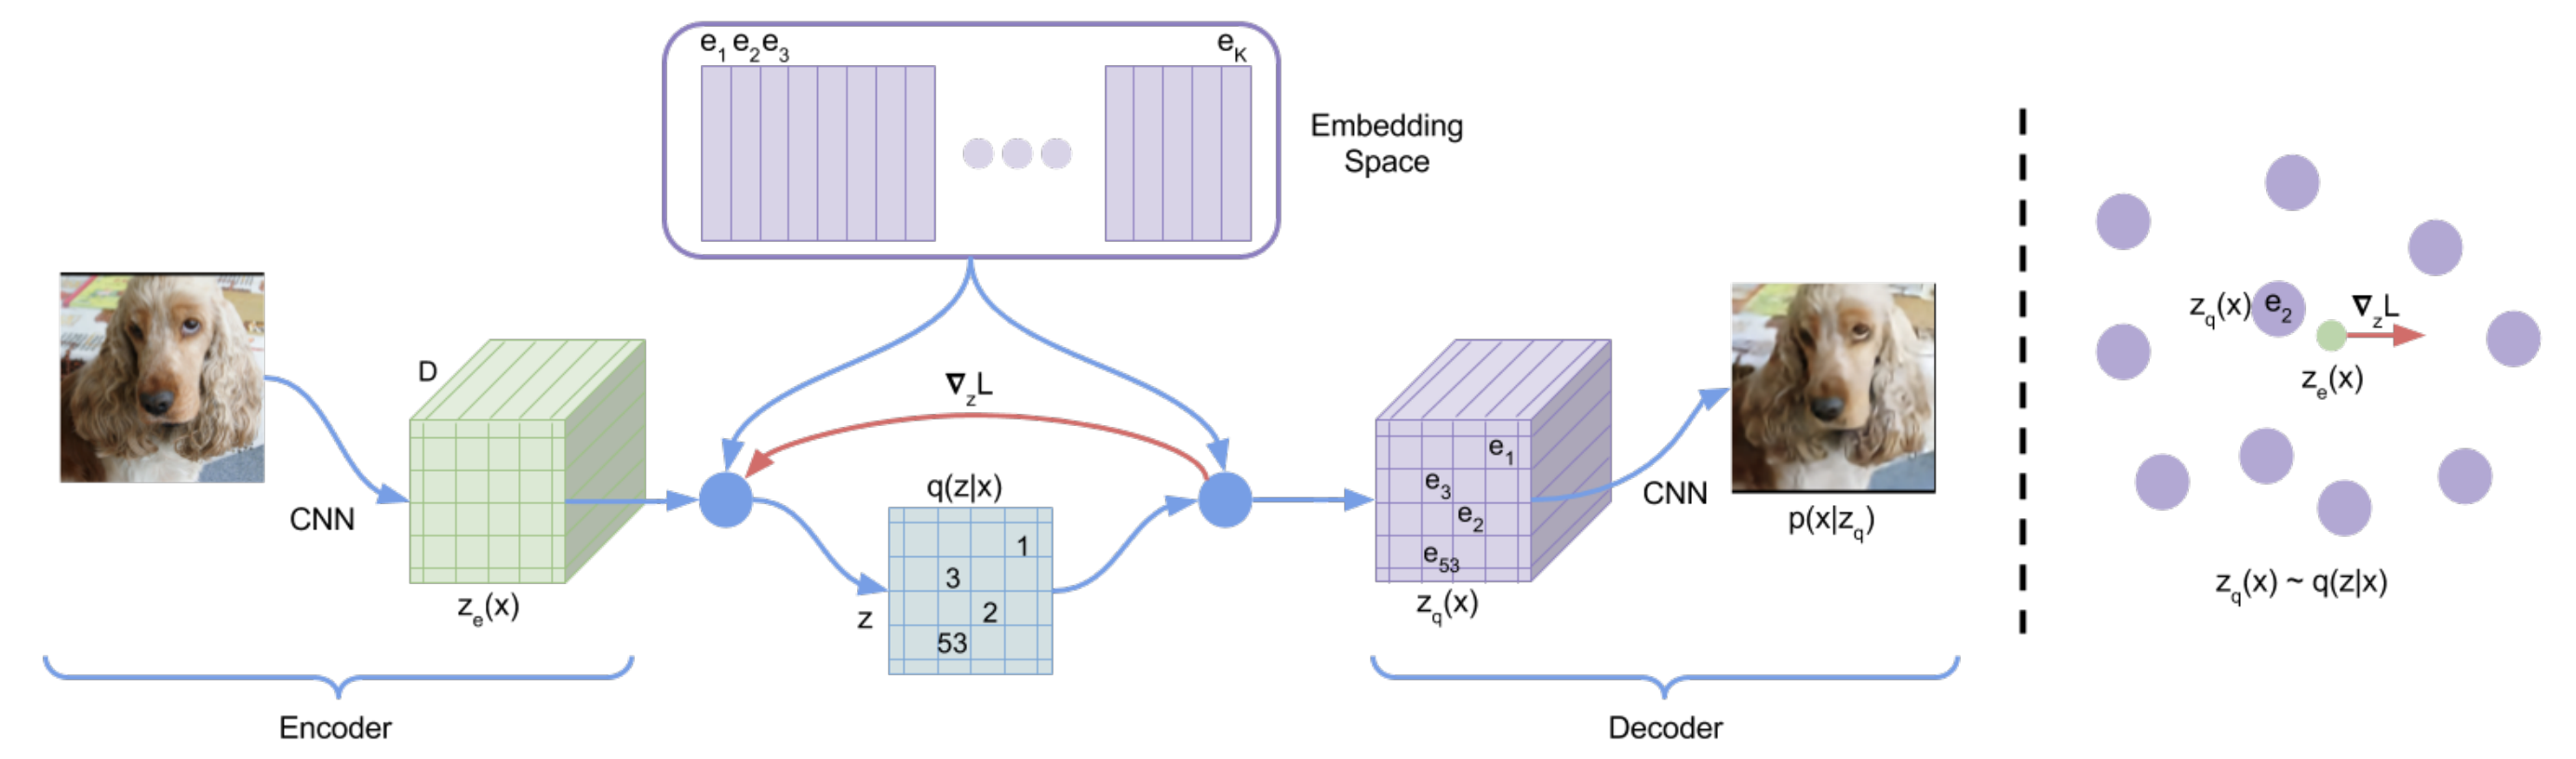
\includegraphics[width=0.85\linewidth]{figs/vqvae}
	\end{figure}
	\vspace{-0.3cm}
	\begin{block}{Deterministic variational posterior}
		\vspace{-0.8cm}
		\[
			q(c_{ij} = k^* | \bx, \bphi) = \begin{cases}
				1 , \quad \text{for } k^* = \argmin_k \| [\bz_e]_{ij} - \be_k \|; \\
				0, \quad \text{otherwise}.
			\end{cases}
		\]
		\vspace{-0.8cm}
	\end{block}
	\begin{block}{ELBO}
		\vspace{-0.6cm}
		\[
			\mathcal{L} (\bphi, \btheta)  = \mathbb{E}_{q(c | \bx, \bphi)} \log p(\bx | \be_{c} , \btheta) - \log K =  \log p(\bx | \bz_q, \btheta) - \log K.
		\]
		\vspace{-0.6cm}
	\end{block}
	\begin{block}{Straight-through gradient estimation}
		\vspace{-0.6cm}
		\[
			\frac{\partial \log p(\bx | \bz_q , \btheta)}{\partial \bphi} = \frac{\partial \log p(\bx | \bz_q, \btheta)}{\partial \bz_q} \cdot {\color{red}\frac{\partial \bz_q}{\partial \bphi}} \approx \frac{\partial \log p(\bx | \bz_q, \btheta)}{\partial \bz_q} \cdot \frac{\partial \bz_e}{\partial \bphi}
		\]
	\end{block}
	\myfootnotewithlink{https://arxiv.org/abs/1711.00937}{Oord A., Vinyals O., Kavukcuoglu K. Neural Discrete Representation Learning, 2017} 
\end{frame}
%=======
\begin{frame}{Recap of previous lecture}
	\vspace{-0.4cm}
	\begin{block}{Gumbel-max trick}
		Let $g_k \sim \text{Gumbel}(0, 1)$ for $k = 1, \dots, K$. Then
		\vspace{-0.3cm}
		\[
			c = \argmax_k [\log \pi_k + g_k]
		\]
		\vspace{-0.6cm} \\
		has a categorical distribution $c \sim \text{Categorical}(\bpi)$.
	\end{block}
	\vspace{-0.2cm}
	\begin{block}{Gumbel-softmax relaxation}
		{\color{violet}Con}{\color{teal}crete} distribution = {\color{violet}\textbf{con}tinuous} + {\color{teal}dis\textbf{crete}}
		\[
			\hat{\bc} = \text{Softmax}\left(\frac{\log q(\bc | \bx, \bphi) + \bg}{\color{olive}\tau}\right)
		\]
		\vspace{-0.7cm}
 	\end{block}
	\begin{block}{Reparametrization trick}
		\vspace{-0.4cm}
		\[
			\nabla_{\bphi} \mathbb{E}_{q(c | \bx, \bphi)} \log p(\bx | \be_{c} , \btheta) = \bbE_{\text{Gumbel}(0, 1)} \nabla_{\bphi} \log p(\bx | \bz , \btheta),
		\]
		where $\bz = \sum_{k=1}^K\hat{c}_k \be_k$ (all operations are differentiable now).
	\end{block}
 	\vspace{-0.2cm}
	\myfootnote{
	\href{https://arxiv.org/abs/1611.00712}{Maddison C. J., Mnih A., Teh Y. W. The Concrete distribution: A continuous relaxation of discrete random variables, 2016} \\
	\href{https://arxiv.org/abs/1611.01144}{Jang E., Gu S., Poole B. Categorical reparameterization with Gumbel-Softmax, 2016}
	}
\end{frame}
%=======
\begin{frame}{Recap of previous lecture}
	\begin{block}{Theorem}
		\vspace{-0.6cm}
		\[
			\frac{1}{n} \sum_{i=1}^n KL(q(\bz | \bx_i, \bphi) || p(\bz)) = KL({\color{teal}q_{\text{agg}}(\bz | \bphi) }|| p(\bz)) + \bbI_{q} [\bx, \bz].
		\]
		\vspace{-0.6cm}
	\end{block}
	\begin{block}{ELBO surgery}
		\vspace{-0.5cm}
		{\small
		\[
		    \frac{1}{n} \sum_{i=1}^n \cL_i(\bphi, \btheta) = \underbrace{\frac{1}{n} \sum_{i=1}^n \mathbb{E}_{q(\bz | \bx_i, \bphi)} \log p(\bx_i | \bz, \btheta)}_{\text{Reconstruction loss}}
		    - \underbrace{\vphantom{ \sum_{i=1}^n} \bbI_q [\bx, \bz]}_{\text{MI}} - \underbrace{\vphantom{ \sum_{i=1}^n} KL({\color{teal}q_{\text{agg}}(\bz | \bphi)} || {\color{violet}p(\bz)})}_{\text{Marginal KL}}
		\]}
	\end{block}
	\vspace{-0.7cm}
	\begin{block}{Optimal prior}
		\vspace{-0.7cm}
		\[
			KL(q_{\text{agg}}(\bz | \bphi) || p(\bz)) = 0 \quad \Leftrightarrow \quad p (\bz) = q_{\text{agg}}(\bz) = \frac{1}{n} \sum_{i=1}^n q(\bz | \bx_i, \bphi).
		\]
		\vspace{-0.5cm}\\
		The optimal prior distribution $p(\bz)$ is the aggregated variational posterior distribution $q_{\text{agg}}(\bz | \bphi)$.
	\end{block}
	\myfootnotewithlink{http://approximateinference.org/accepted/HoffmanJohnson2016.pdf}{Hoffman M. D., Johnson M. J. ELBO surgery: yet another way to carve up the variational evidence lower bound, 2016}
\end{frame}
%=======
\begin{frame}{Outline}
	\tableofcontents
\end{frame}
%=======
\section{Learnable VAE prior}
%=======
\begin{frame}{Optimal VAE prior}
	\begin{itemize}
		\item Standard Gaussian $p(\bz) = \mathcal{N}(0, \bI)$ $\Rightarrow$ over-regularization;
		\item $p(\bz) = q_{\text{agg}}(\bz | \bphi) = \frac{1}{n}\sum_{i=1}^n q(\bz | \bx_i, \bphi)$ $\Rightarrow$ overfitting and highly expensive.
	\end{itemize}
	\vspace{-0.5cm}
	\begin{minipage}[t]{0.5\columnwidth}
		\begin{block}{Non learnable prior $p(\bz)$}
			\begin{figure}[h]
				\centering
				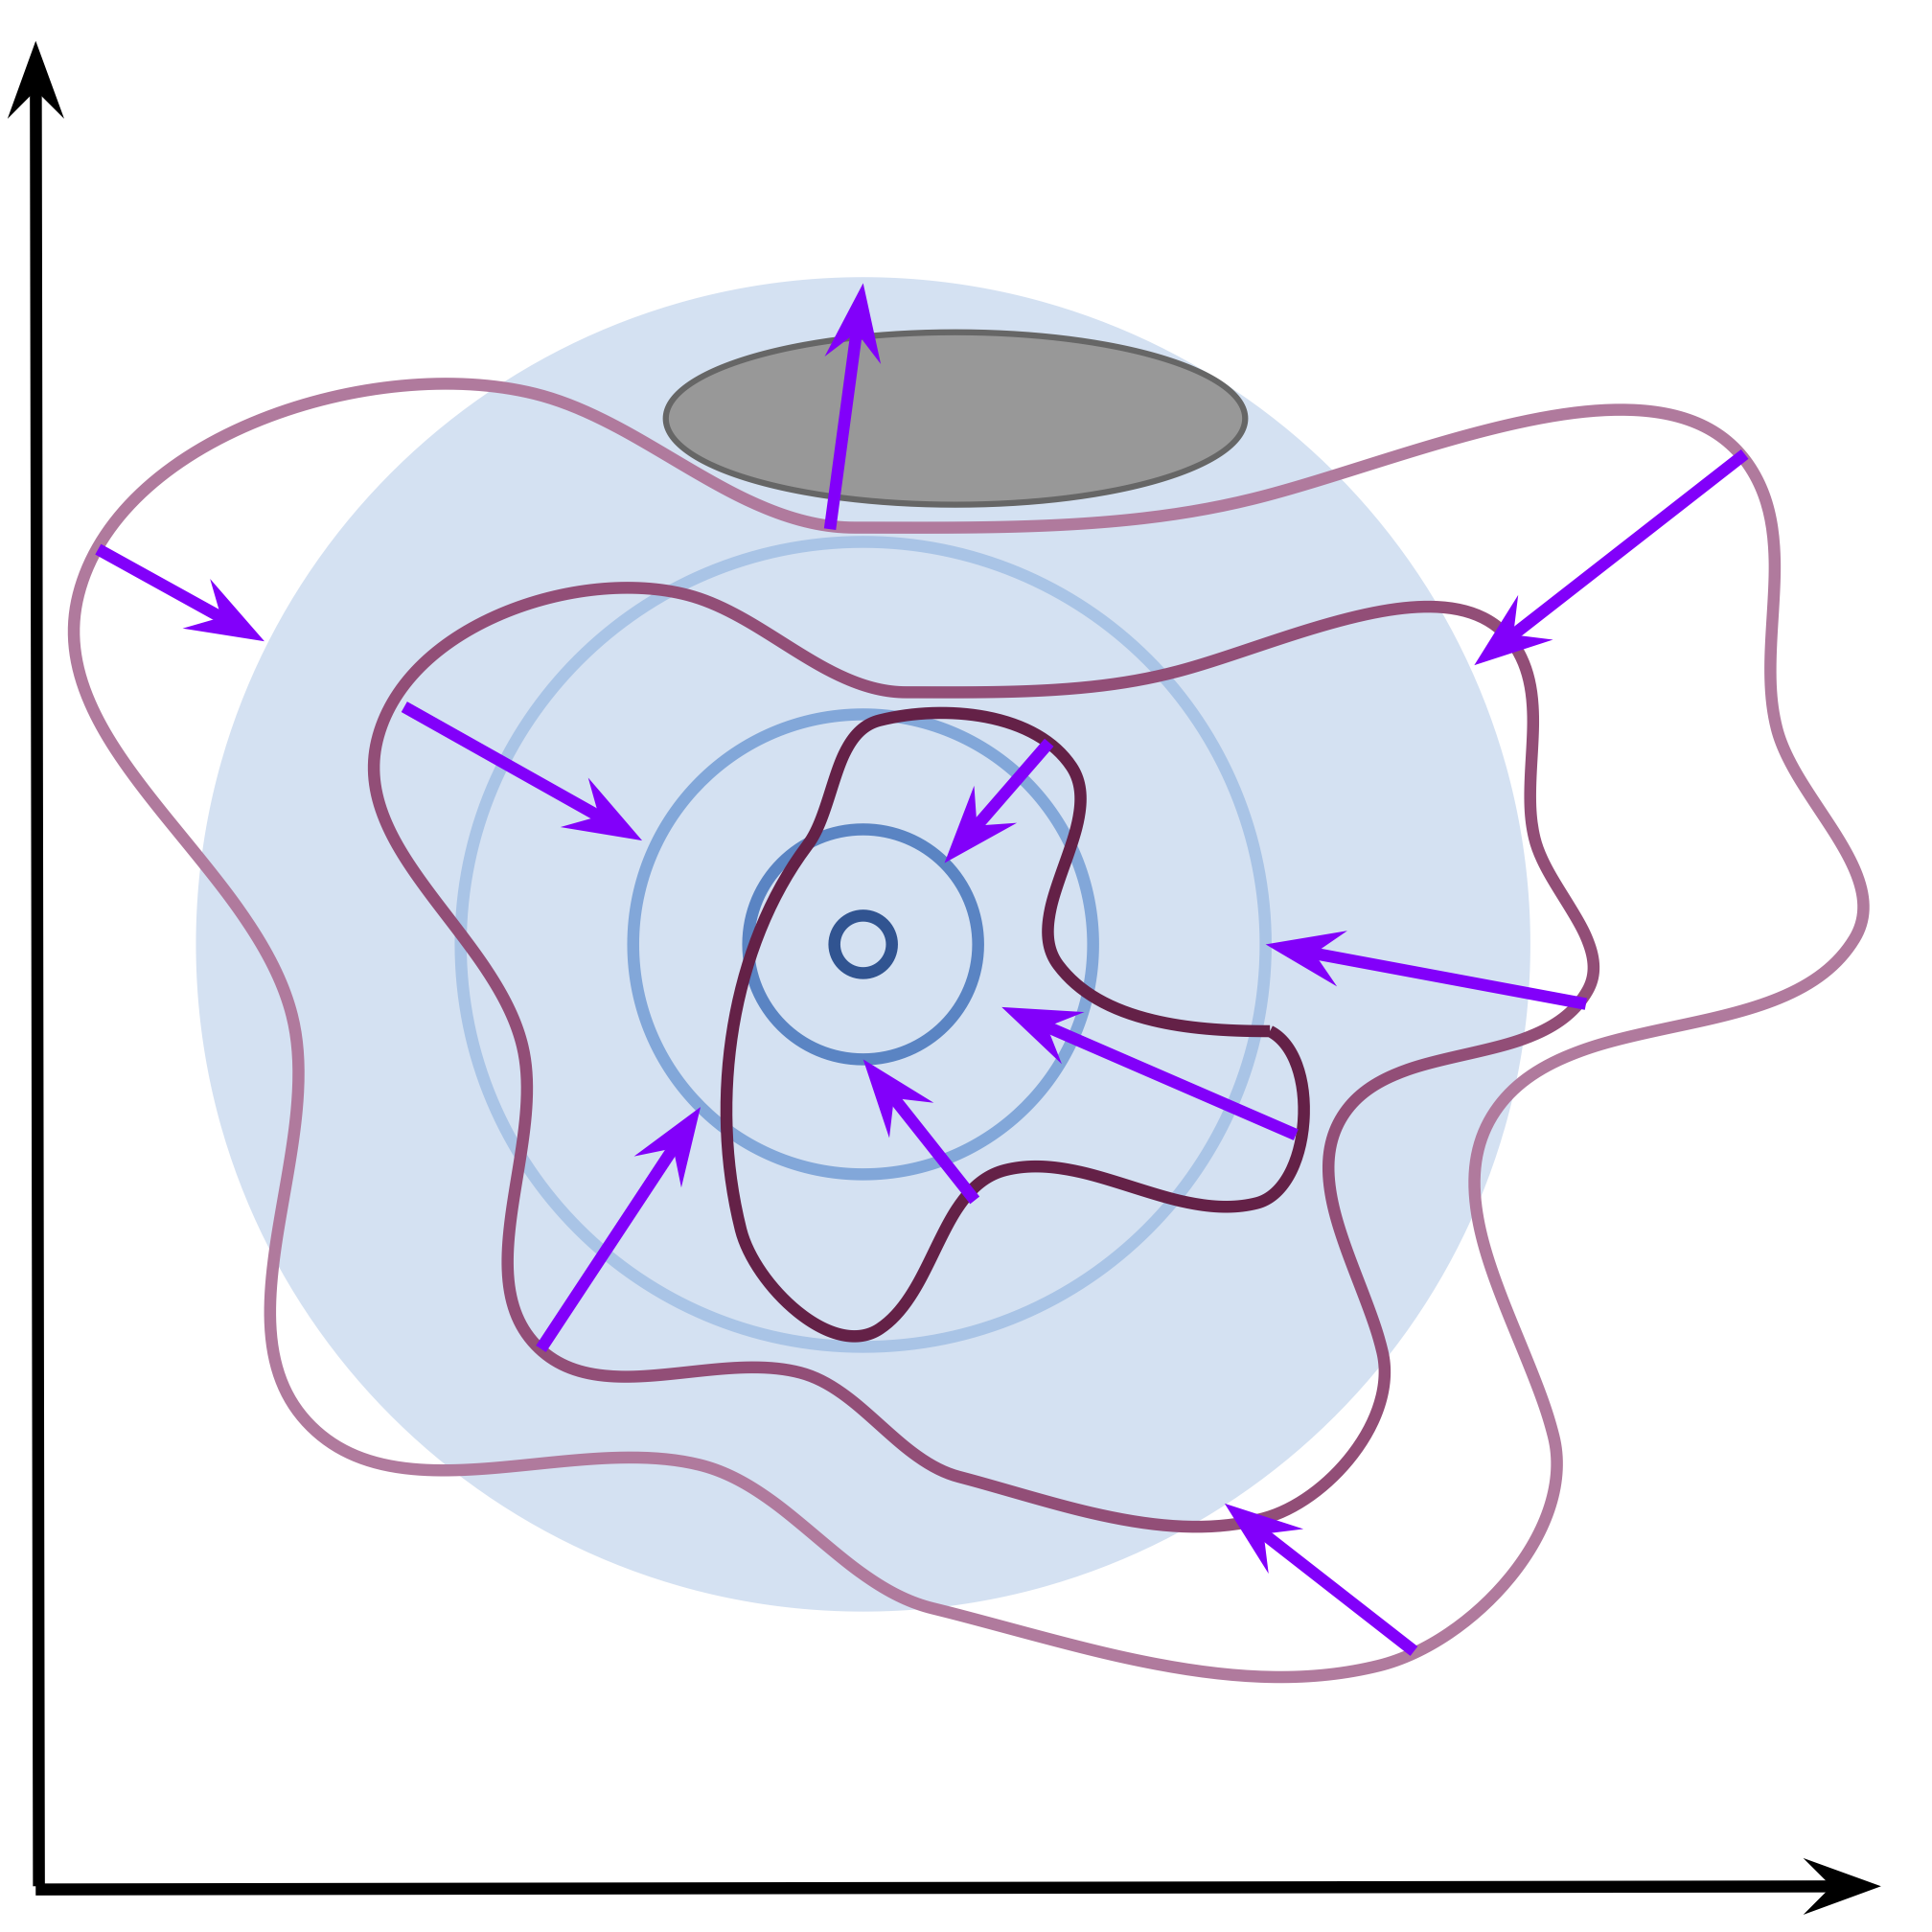
\includegraphics[width=0.6\linewidth]{figs/non_learnable_prior}
			\end{figure}
		\end{block}
	\end{minipage}%
	\begin{minipage}[t]{0.5\columnwidth}
		\begin{block}{Learnable prior $p(\bz | \blambda)$}
			\begin{figure}[h]
				\centering
				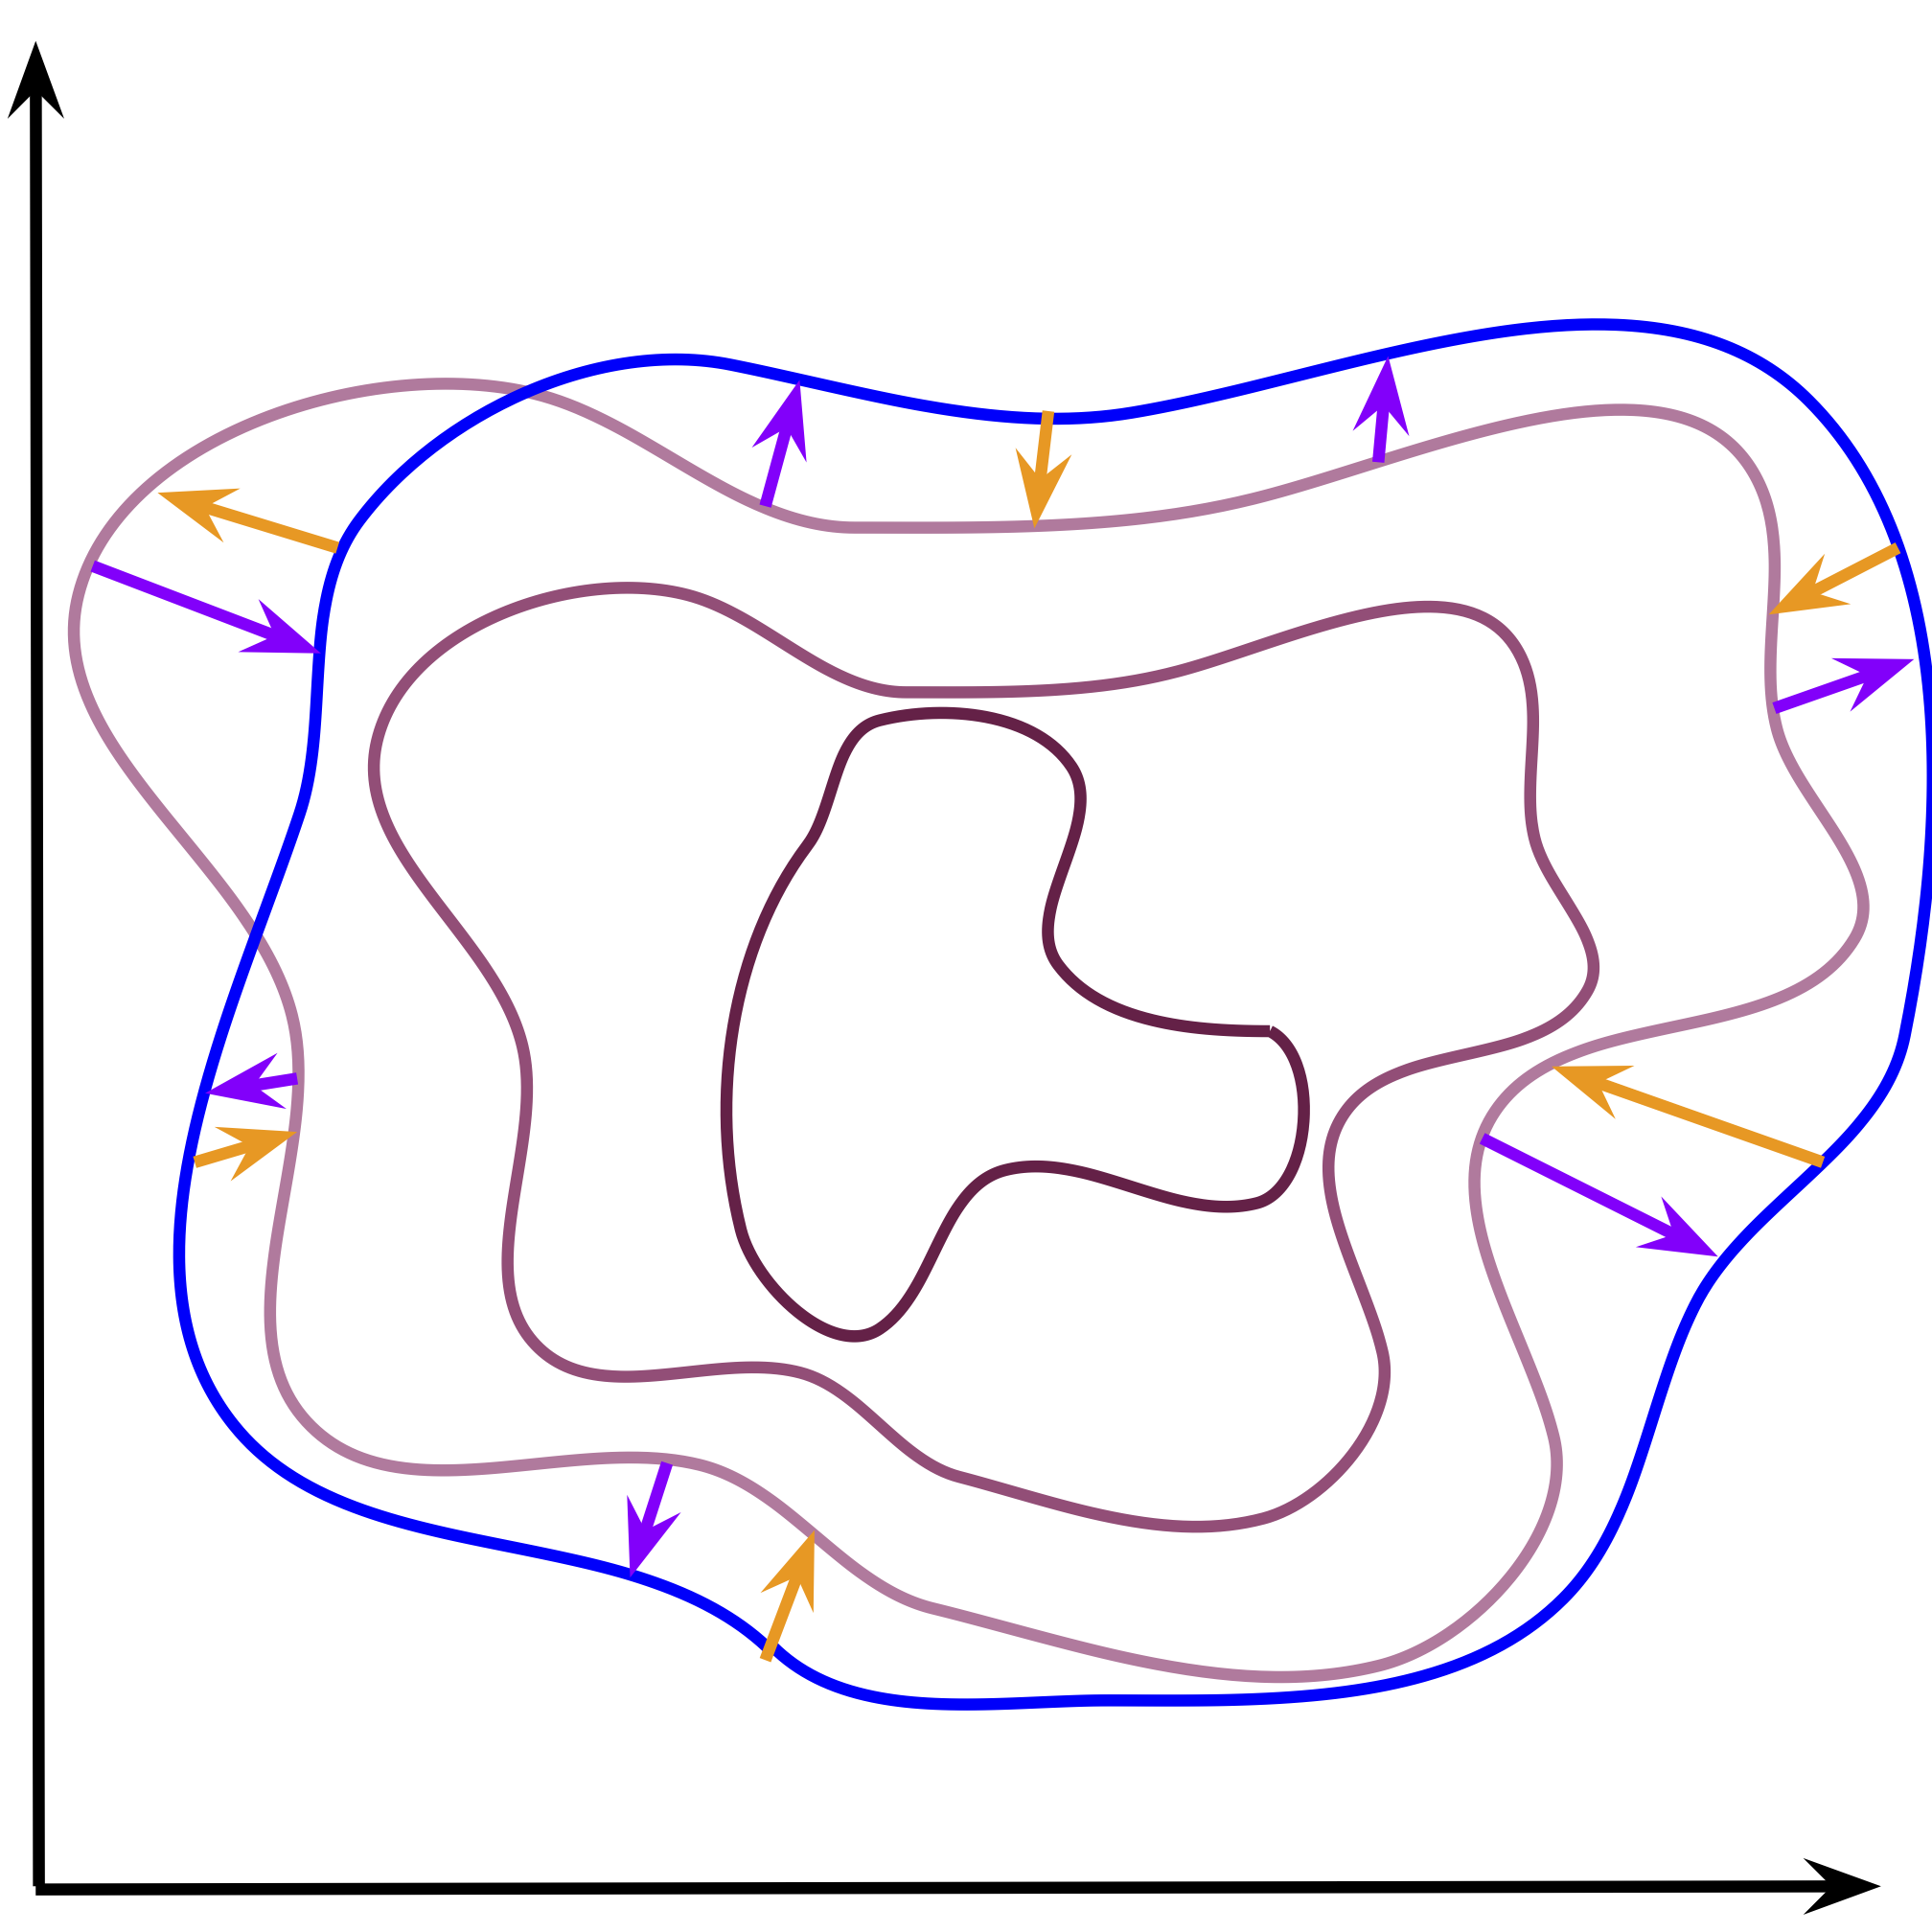
\includegraphics[width=0.6\linewidth]{figs/learnable_prior}
			\end{figure}
		\end{block}
	\end{minipage}
	\vspace{-0.4cm}
	\begin{block}{ELBO revisiting}
		\vspace{-0.3cm}
		\[
		\frac{1}{n}\sum_{i=1}^n \cL_i(\bphi, \btheta) = \text{RL} - \text{MI} -  KL(q_{\text{agg}}(\bz | \bphi) || {\color{teal}p(\bz | \blambda)})
		\]
		It is Forward KL with respect to $p(\bz | \blambda)$.
	\end{block}
	\myfootnotewithlink{https://jmtomczak.github.io/blog/7/7\_priors.html}{image credit: https://jmtomczak.github.io/blog/7/7\_priors.html}
\end{frame}
%=======
\begin{frame}{NF-based VAE prior}
	\begin{block}{NF model in latent space}
		\vspace{-0.5cm}
		\[
		\log p(\bz | \blambda) = \log p(\bz^*) + \log  \left | \det \left(\frac{d \bz^*}{d\bz}\right)\right| = \log p(\bff_{\blambda}(\bz)) + \log \left | \det (\bJ_\bff)\right| 
		\]
		\vspace{-0.3cm}
		\[
		\bz = \bg_{\blambda}(\bz^*) = \bff^{-1}_{\blambda}(\bz^*)
		\]
	\end{block}
	\vspace{-0.3cm}
	\begin{itemize}
		\item RealNVP with coupling layers.
		\item Autoregressive NF (fast $\bff_{\blambda}(\bz)$, slow $\bg_{\blambda}(\bz^*)$).
	\end{itemize}
	\begin{block}{ELBO with NF-based VAE prior}
		\vspace{-0.5cm}
		{\small
			\begin{multline*}
				\mathcal{L}(\bphi, \btheta) = \mathbb{E}_{q(\bz | \bx, \bphi)} \left[ \log p(\bx | \bz, \btheta) + {\color{violet}\log p(\bz | \blambda)} - \log q(\bz | \bx, \bphi) \right] \\
				= \mathbb{E}_{q(\bz | \bx, \bphi)} \Bigl[ \log p(\bx | \bz, \btheta) + \underbrace{ \Bigl({\color{violet} \log p(\bff_{\blambda}(\bz)) + \log \left| \det (\bJ_\bff) \right|} \Bigr) }_{\text{NF-based prior}} - \log q(\bz | \bx, \bphi) \Bigr] 
			\end{multline*}
		}
	\end{block}
	\myfootnotewithlink{https://arxiv.org/abs/1611.02731}{Chen X. et al. Variational Lossy Autoencoder, 2016}
\end{frame}
%=======
\section{Likelihood-free learning}
%=======
\begin{frame}{Likelihood based models}
	\begin{minipage}[t]{0.48\columnwidth}
		\begin{block}{Poor likelihood \\ Great samples}
			\vspace{-0.3cm}
			\[
				p_1(\bx) = \frac{1}{n} \sum_{i=1}^n \cN(\bx | \bx_i, \epsilon \bI)
			\]
			For small $\epsilon$ this model will generate samples with great quality, but likelihood of test sample will be very poor.
		\end{block}
	\end{minipage}%
	\begin{minipage}[t]{0.52\columnwidth}
		\begin{block}{Great likelihood \\ Poor samples}
			\vspace{-0.3cm}
			\[
				p_2(\bx) = 0.01p(\bx) + 0.99p_{\text{noise}}(\bx)
			\]
			\begin{multline*}
				\log \left[ 0.01p(\bx) + 0.99p_{\text{noise}}(\bx) \right] \geq  \\ \geq \log \left[ 0.01p(\bx) \right]  = \log p(\bx) - \log 100
			\end{multline*}
		Noisy irrelevant samples, but for high dimensions $\log p(\bx)$ becomes proportional to $m$.
		\end{block}
	\end{minipage}
	\begin{itemize}
		\item Likelihood is not a perfect quality measure for generative model.
		\item Likelihood could be intractable.
	\end{itemize}
	\myfootnotewithlink{https://arxiv.org/abs/1511.01844}{Theis L., Oord A., Bethge M. A note on the evaluation of generative models, 2015}
\end{frame}
%=======
\begin{frame}{Likelihood-free learning}
	\begin{block}{Where did we start}
	 We would like to approximate true data distribution $\pi(\bx)$.
	Instead of searching true $\pi(\bx)$ over all probability distributions, learn function approximation $p(\bx | \btheta) \approx \pi(\bx)$.
	\end{block}
	Imagine we have two sets of samples 
	\begin{itemize}
		\item $\cS_1 = \{\bx_i\}_{i=1}^{n_1} \sim \pi(\bx)$ -- real samples;
		\item $\cS_2 = \{\bx_i\}_{i=1}^{n_2} \sim p(\bx | \btheta)$ -- generated (or fake) samples.
	\end{itemize}
	Let define discriminative model (classifier):
	\[
		p(y = 1 | \bx) = P\bigl(\{\bx \sim \pi(\bx)\}\bigr); \quad p(y = 0 | \bx) = P\bigl(\{\bx \sim p(\bx | \btheta)\}\bigr)
	\]
	\vspace{-0.5cm}
	\begin{block}{Assumption}
		Generative distribution $p(\bx | \btheta)$ equals to the true distribution $\pi(\bx)$ if we can not distinguish them using discriminative model $p(y | \bx)$. \\
		It means that $p(y = 1 | \bx) = 0.5$ for each sample $\bx$.
	\end{block}

\end{frame}
%=======
\begin{frame}{Generative adversarial networks (GAN)}
	The more powerful discriminative model we will have, the more likely we will get the "best" generative distribution $p(\bx | \btheta)$. \\
	The most common way to learn a classifier is to minimize cross entropy loss.
	\begin{itemize}
		\item \textbf{Generator:} generative model $\bx = \bG(\bz)$, which makes generated sample more realistic. Here $\bz$ comes from the base (known) distribution $p(\bz)$ and $\bx \sim p(\bx | \btheta)$. Generator tries to \textbf{maximize} cross entropy.
		\item \textbf{Discriminator:} a classifier $p(y = 1 | \bx) = D(\bx) \in [0, 1]$, which distinguishes real samples from generated samples. Discriminator tries to \textbf{minimize} cross entropy (tries to enhance discriminative model).
	\end{itemize}
	\begin{block}{Objective}
		\vspace{-0.5cm}
		\[
			\min_{G} \max_D \left[ \bbE_{\pi(\bx)} \log D(\bx) + \bbE_{p(\bx | \btheta)} \log (1 - D(\bx)) \right] 
		\]
		\[
			\min_{G} \max_D \left[ \bbE_{\pi(\bx)} \log D(\bx) + \bbE_{p(\bz)} \log (1 - D(\bG(\bz))) \right]
		\]
	\end{block}
	\myfootnotewithlink{https://arxiv.org/abs/1406.2661}{Goodfellow I. J. et al. Generative Adversarial Networks, 2014}
\end{frame}
%=======
\section{Generative adversarial networks (GAN)}
%=======
\begin{frame}{Generative models zoo}
	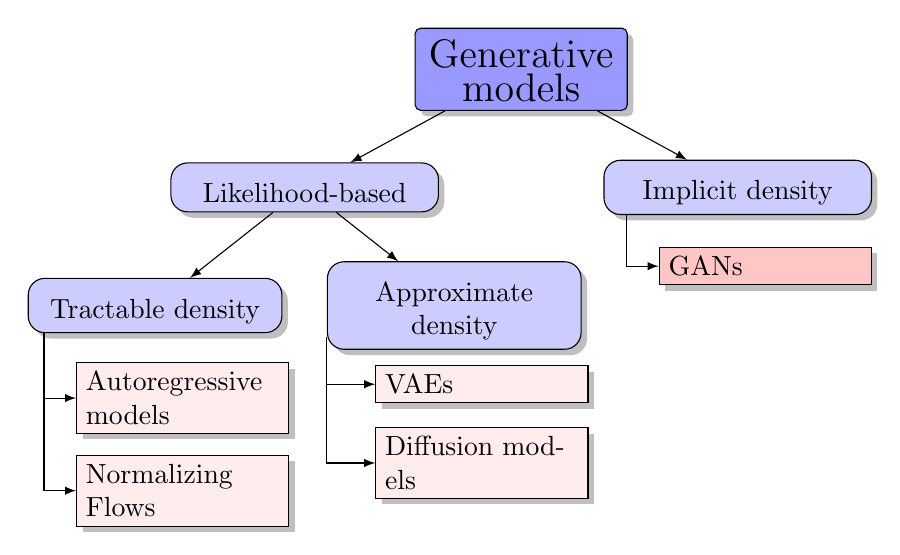
\begin{tikzpicture}[
	 	basic/.style  = {draw, text width=2cm, drop shadow, rectangle},
	 	root/.style   = {basic, rounded corners=2pt, thin, text height=1.1em, text width=7em, align=center, fill=blue!40},
	 	level 1/.style={sibling distance=55mm},
	 	level 2/.style = {basic, rounded corners=6pt, thin, align=center, fill=blue!20, text height=1.1em, text width=9em, sibling distance=38mm},
	 	level 3/.style = {basic, rounded corners=6pt, thin,align=center, fill=blue!20, text width=8.5em},
	 	level 4/.style = {basic, thin, align=left, fill=pink!30, text width=7em},
	 	level 5/.style = {basic, thin, align=left, fill=pink!90, text width=7em},
		edge from parent/.style={->,draw},
		>=latex]
		
		% root of the the initial tree, level 1
		\node[root] {\Large Generative models}
		% The first level, as children of the initial tree
		child {node[level 2] (c1) {Likelihood-based}
			child {node[level 3] (c11) {Tractable density}}
			child {node[level 3] (c12) {Approximate density}}
		}
		child {node[level 2] (c2) {Implicit density}};
		
		% The second level, relatively positioned nodes
		\begin{scope}[every node/.style={level 4}]
		\node [below of = c11, yshift=-5pt, xshift=10pt] (c111) {Autoregressive models};
		\node [below of = c111, yshift=-5pt] (c112) {Normalizing Flows};
		
		\node [below of = c12, xshift=10pt] (c121) {VAEs};
		\node [below of = c121] (c122) {Diffusion models};
		
		\end{scope}
		
		% The second level, relatively positioned nodes
		\begin{scope}[every node/.style={level 5}]
		\node [below of = c2, xshift=10pt] (c21) {GANs};
		\end{scope}
		
		
		% lines from each level 1 node to every one of its "children"
		\foreach \value in {1,2}
		\draw[->] (c11.194) |- (c11\value.west);
		
		\foreach \value in {1,2}
		\draw[->] (c12.194) |- (c12\value.west);
		
		\draw[->] (c2.194) |- (c21.west);
		
	\end{tikzpicture}
\end{frame}
%=======
\begin{frame}{GAN optimality}
	\begin{block}{Theorem}
		The minimax game 
		\vspace{-0.3cm}
		\[
			\min_{G} \max_D \Bigl[ \underbrace{\bbE_{\pi(\bx)} \log D(\bx) + \bbE_{p(\bz)} \log (1 - D(\bG(\bz)))}_{V(G, D)} \Bigr]
		\]
		\vspace{-0.5cm} \\
		has the global optimum $\pi(\bx) = p(\bx | \btheta)$, in this case $D^*(\bx) = 0.5$.
	\end{block}
	\begin{block}{Proof (fixed $G$)}
		\vspace{-0.5cm}
		\begin{align*}
			V(G, D) &= \bbE_{\pi(\bx)} \log D(\bx) + \bbE_{p(\bx | \btheta)} \log (1 - D(\bx)) \\
			&= \int \underbrace{\left[ \pi(\bx) \log D(\bx) + p(\bx | \btheta)\log (1 - D(\bx) \right]}_{y(D)} d \bx
		\end{align*}
		\vspace{-0.2cm}
		\[
			\frac{d y(D)}{d D} = \frac{\pi(\bx)}{D(\bx)} - \frac{p(\bx | \btheta)}{1 - D(\bx)} = 0 \quad \Rightarrow \quad D^*(\bx) = \frac{\pi(\bx)}{\pi(\bx) + p(\bx | \btheta)}
		\]
	\end{block}
	\myfootnotewithlink{https://arxiv.org/abs/1406.2661}{Goodfellow I. J. et al. Generative Adversarial Networks, 2014}
\end{frame}
%=======
\begin{frame}{GAN optimality}
	\begin{block}{Proof continued (fixed $D = D^*$)}
		\vspace{-0.5cm}
		\begin{multline*}
			V(G, D^*) = \bbE_{\pi(\bx)} \log \left( \frac{\pi(\bx)}{\pi(\bx) + p(\bx | \btheta)} \right) + \bbE_{p(\bx | \btheta)} \log \left( \frac{p(\bx | \btheta)}{\pi(\bx) + p(\bx | \btheta)}\right)  \\
		 = KL \left(\pi(\bx) || \frac{\pi(\bx) + p(\bx | \btheta)}{2}\right) + KL \left(p(\bx | \btheta) || \frac{\pi(\bx) + p(\bx | \btheta)}{2}\right) - 2\log 2 \\
		 = 2JSD(\pi(\bx) || p(\bx | \btheta)) - 2\log 2.
		\end{multline*}
	\end{block}
	\vspace{-0.3cm}
	\begin{block}{Jensen-Shannon divergence (symmetric KL divergence)}
		\vspace{-0.2cm}
		\footnotesize
		\[
			JSD(\pi(\bx) || p(\bx | \btheta)) = \frac{1}{2} \left[KL \left(\pi(\bx) || \frac{\pi(\bx) + p(\bx | \btheta)}{2}\right) + KL \left(p(\bx | \btheta) || \frac{\pi(\bx) + p(\bx | \btheta)}{2}\right) \right]
		\]
	\end{block}
	Could be used as a distance measure!
	\[
		V(G^*, D^*) = -2\log 2, \quad \pi(\bx) = p(\bx | \btheta), \quad  D^*(\bx) = 0.5.
	\]
	
	 \myfootnotewithlink{https://arxiv.org/abs/1406.2661}{Goodfellow I. J. et al. Generative Adversarial Networks, 2014}
\end{frame}
%=======
\begin{frame}{GAN optimality}
	\begin{block}{Theorem}
		The minimax game 
		\vspace{-0.3cm}
		\[
		\min_{G} \max_D \Bigl[ \underbrace{\bbE_{\pi(\bx)} \log D(\bx) + \bbE_{p(\bz)} \log (1 - D(\bG(\bz)))}_{V(G, D)} \Bigr]
		\]
		\vspace{-0.5cm} \\
		has the global optimum $\pi(\bx) = p(\bx | \btheta)$, in this case $D^*(\bx) = 0.5$.
	\end{block}
	\vspace{-0.2cm}
	\begin{block}{Expectations}
		If the generator could be \textbf{any} function and the discriminator is \textbf{optimal} at every step, then the generator is \textbf{guaranteed to converge} to the data distribution.
	\end{block}
	\begin{block}{Reality}
		\begin{itemize}
			\item Generator updates are made in parameter space, discriminator is not optimal at every step.
			\item Generator and discriminator loss keeps oscillating during GAN training.
		\end{itemize}
	\end{block}
	 \myfootnotewithlink{https://arxiv.org/abs/1406.2661}{Goodfellow I. J. et al. Generative Adversarial Networks, 2014}
\end{frame}
%=======
\begin{frame}{GAN training}
	Let further assume that generator and discriminator are parametric models: $D_{\bphi}(\bx)$ and $\bG_{\btheta}(\bz)$.
	\begin{block}{Objective}
		\vspace{-0.7cm}
		\[
		\min_{\btheta} \max_{\bphi} \left[ \bbE_{\pi(\bx)} \log D_{\bphi}(\bx) + \bbE_{p(\bz)} \log (1 - D_{\bphi}(\bG_{\btheta}(\bz))) \right]
		\]
		\vspace{-0.7cm}
	\end{block}
	\begin{figure}
		\centering
		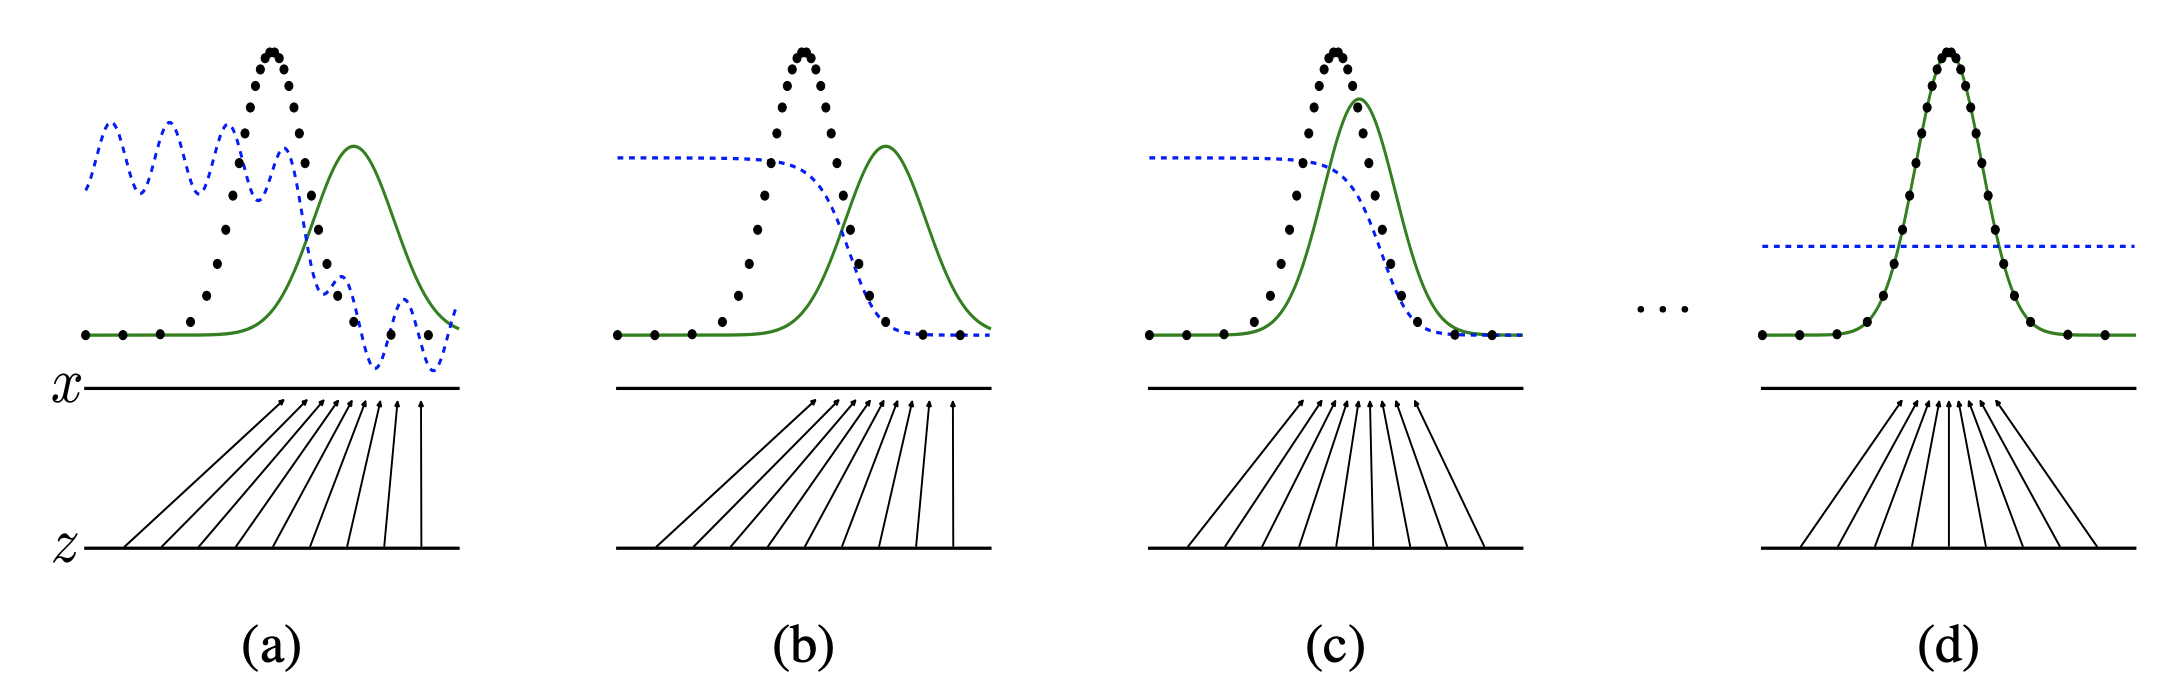
\includegraphics[width=1.0\linewidth]{figs/gan_1}
	\end{figure}

	\begin{itemize}
		\item $\bz \sim p(\bz)$ is a latent variable.
		\item $p(\bx | \bz, \btheta) = \delta(\bx - \bG_{\btheta}(\bz))$ is deterministic decoder ({\color{gray} like NF}).
		\item We do not have encoder at all.
	\end{itemize}

	 \myfootnotewithlink{https://arxiv.org/abs/1406.2661}{Goodfellow I. J. et al. Generative Adversarial Networks, 2014}
\end{frame}
%=======
\begin{frame}{Mode collapse}
	The phenomena where the generator of a GAN collapses to one or few distribution modes.
	\vspace{-0.15cm}
	\begin{figure}
		\centering
		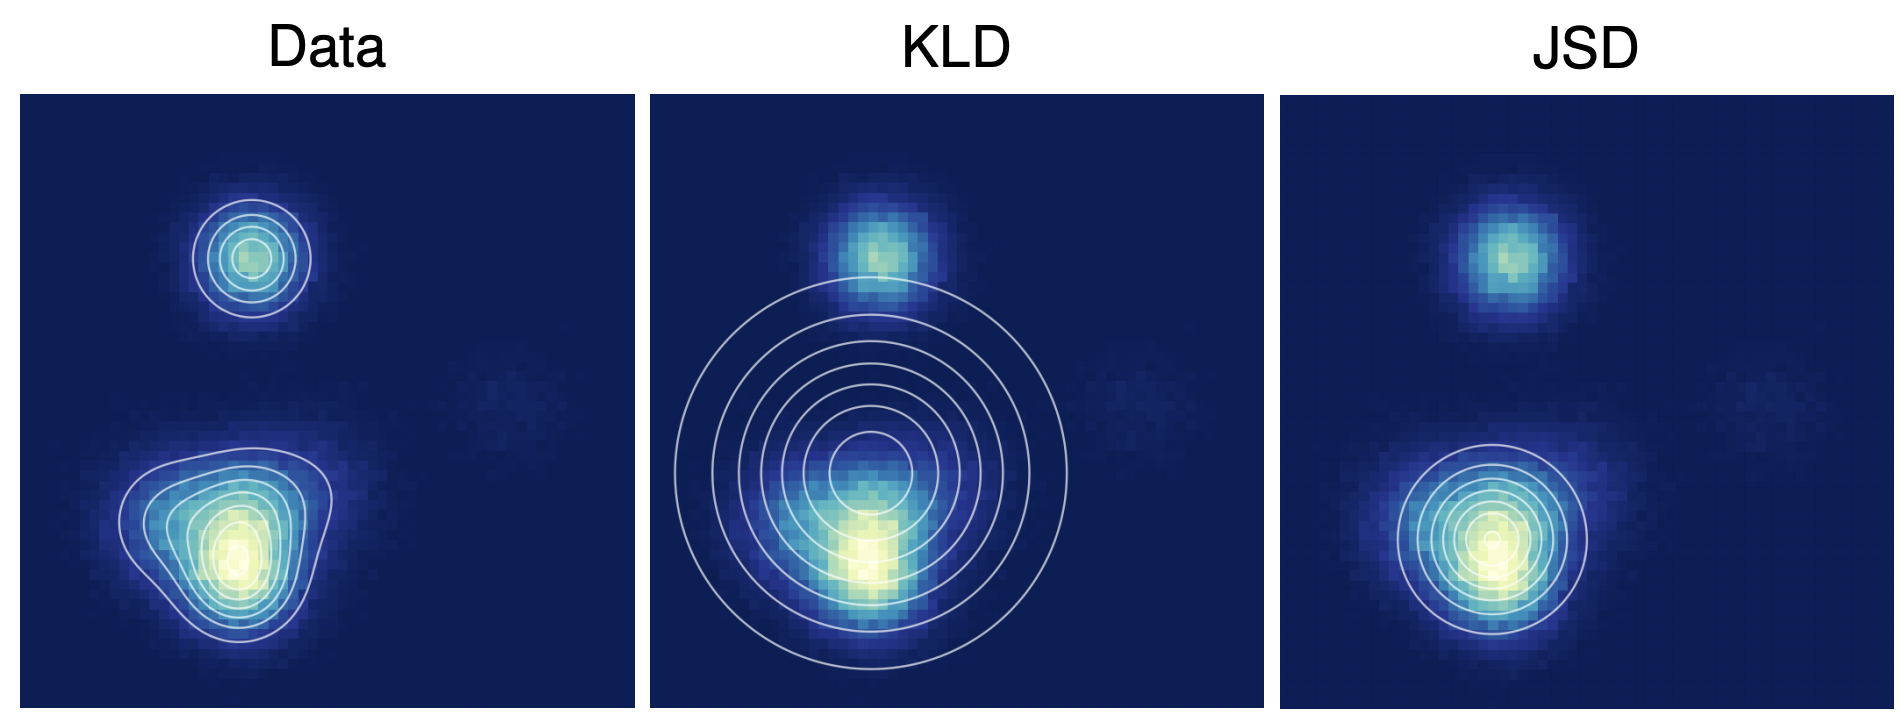
\includegraphics[width=0.75\linewidth]{figs/mode_collapse_1}
	\end{figure}
	\vspace{-0.3cm}
	\begin{figure}
		\centering
		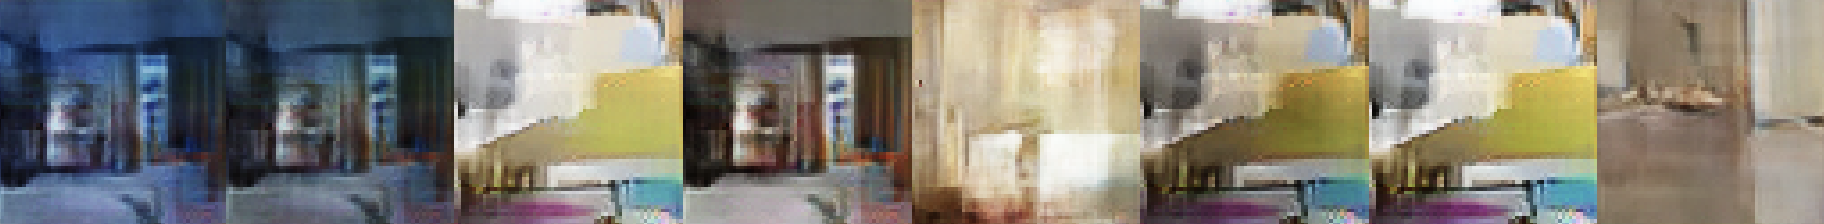
\includegraphics[width=1.0\linewidth]{figs/mode_collapse_4}
	\end{figure}
	Alternate architectures, adding regularization terms, injecting small noise
	perturbations and other millions bags and tricks are used to avoid the mode collapse.
	
	\myfootnote{\href{https://arxiv.org/abs/1406.2661}{Goodfellow I. J. et al. Generative Adversarial Networks, 2014} \\
		\href{https://arxiv.org/abs/1611.02163}{Metz L. et al. Unrolled Generative Adversarial Networks, 2016}}
\end{frame}
%=======
\begin{frame}{Jensen-Shannon vs Kullback-Leibler }
	\begin{itemize}
		\item $\pi(\bx)$ is a fixed mixture of 2 gaussians.
		\item $p(\bx | \mu, \sigma) = \cN(\mu, \sigma^2)$.
	\end{itemize}
	\begin{block}{Mode covering vs mode seeking}
		\vspace{-0.7cm}
		\[
		KL(\pi || p) = \int \pi(\bx) \log \frac{\pi(\bx)}{p(\bx)}d\bx, \quad KL(p || \pi) = \int p(\bx) \log \frac{p(\bx)}{\pi(\bx)}d\bx
		\]
		\[
		JSD(\pi || p) = \frac{1}{2} \left[KL \left(\pi(\bx) || \frac{\pi(\bx) + p(\bx)}{2}\right) + KL \left(p(\bx) || \frac{\pi(\bx) + p(\bx)}{2}\right) \right]
		\]
		\vspace{-0.7cm}
		
		\begin{minipage}[t]{0.33\columnwidth}
			\begin{figure}
				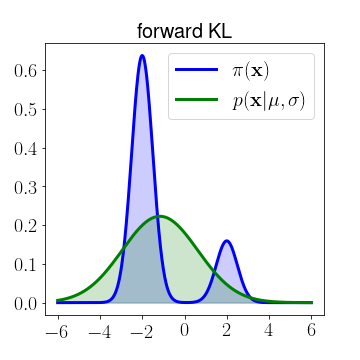
\includegraphics[width=\linewidth]{figs/forward_KL}
			\end{figure}
		\end{minipage}%
		\begin{minipage}[t]{0.33\columnwidth}
			\begin{figure}
				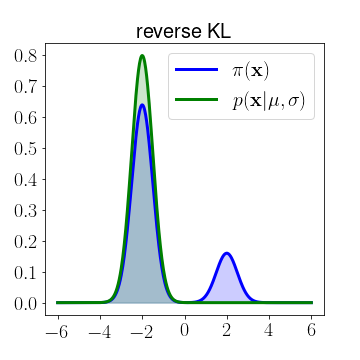
\includegraphics[width=\linewidth]{figs/reverse_KL}
			\end{figure}
		\end{minipage}%
		\begin{minipage}[t]{0.33\columnwidth}
			\begin{figure}
				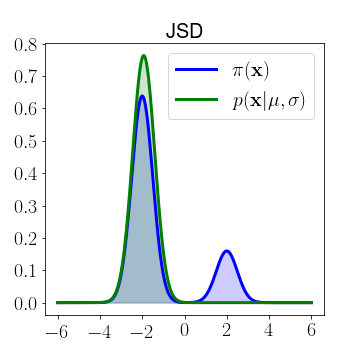
\includegraphics[width=\linewidth]{figs/JSD}
			\end{figure}
		\end{minipage}
		\vspace{-0.3cm}
	\end{block}
\end{frame}
%=======
\begin{frame}{Summary}
	\begin{itemize}
		\item We could use NF-based prior in VAE (even autoregressive).
		\vfill
		\item Likelihood is not a perfect criteria to measure quality of generative model.		
		\vfill
		\item Adversarial learning suggests to solve minimax problem to match the distributions.
		\vfill
		\item GAN tries to optimize Jensen-Shannon divergence (in theory).
		\vfill
		\item Mode collapse is one of the main problems of vanilla GAN.  Lots of tips and tricks has to be used to make the GAN training is stable and scalable.
	\end{itemize}
\end{frame}
\end{document} 